\subsubsection{\stid{3.11} ALExa}


\paragraph{Overview}

The ALExa project ({\sl Accelerated Libraries for Exascale}) focuses on
preparing the DTK and Tasmanian libraries for exascale platforms and
integrating these libraries into ECP applications.  These libraries deliver
capabilities identified as needs of ECP applications: (1) the ability to
transfer computed solutions between grids with differing layouts on parallel
accelerated architectures, enabling multiphysics projects to seamlessly
combine results from different computational grids to perform their required
simulations (DTK); and
%
(2) the ability to construct fast and memory efficient surrogates to large
scale engineering models with multiple inputs and large number of outputs,
enabling uncertainty quantification (both forward and inverse) as well as
optimization and efficient multi-physics simulations in projects such as
ExaStar (Tasmanian).

These capabilities are being developed through ongoing interactions with our
ECP application project collaborators to ensure they will satisfy requirements
of these customers.  The libraries in turn take advantage of other ECP/SW
capabilities currently in development, including Trilinos and ForTrilinos,
Kokkos and SLATE.  The final outcome of the ECP project will be a set of
libraries deployed to facilities and also made broadly available as part of
the xSDK4ECP project.


{\bf DTK} (Data Transfer Kit)

{\it Purpose:} Transfers computed solutions between grids with differing
layouts on parallel accelerated architectures.

{\it Significance:} Coupled applications frequently have different grids with
different parallel distributions; DTK is able to transfer solution values
between these grids efficiently and accurately.

{\it Mesh and mesh-free interpolation capabilities:} multivariate data
interpolation between point clouds and grids; compactly supported radial basis
functions; nearest-neighbor and moving least square implementations; support
for standard finite-element shape functions and user-defined interpolants;
common applications include conjugate heat transfer, fluid structure
interaction, and mesh deformation.

{\it Performance portable search capabilities:} shared memory and GPU
implementations of spatial tree construction; shared memory and GPU
implementations of various spatial tree queries; MPI front-end for
coordinating distributed spatial searches between sets of geometric objects
with different decompositions; communication plan generation based on spatial
search results.

{\it URL:} https://github.com/ORNL-CEES/DataTransferKit


{\bf Tasmanian} (Toolkit for Adaptive Stochastic Modeling and Non-Intrusive
Approximation)

{\it Purpose:} Constructs efficient surrogate models for high dimensional
problems and performs parameter calibration and optimization geared towards
applications in uncertainty quantification (UQ).

{\it Significance:} UQ pertains to the statistical properties of the output
from a complex model with respect to variability in multiple model inputs;
large number of simulations are required to compute reliable statistics which
is prohibitive when dealing with computationally expensive engineering
models. A surrogate model is constructed from a moderate set of simulations
using carefully chosen input values; analysis can then be performed on the
efficient surrogate.

{\it Sparse grids capabilities:} surrogate modeling and design of experiments
(adaptive multi-dimensional interpolation); reduced (lossy) representation of
tabulated scientific data; high dimensional numerical quadrature; data mining
and manifold learning.

{\it DiffeRential Evolution Adaptive Metropolis (DREAM) capabilities:}
Bayesian inference; parameter estimation/calibration; model validation.
global optimization and optimization under uncertainty.

{\it URL:} http://tasmanian.ornl.gov

\paragraph{Key Challenges}

\indent

{\bf DTK:} General data transfer between grids of unrelated applications
requires many-to-many communication which is increasingly challenging as
communication to computation ratios are decreasing on successive HPC systems.
Search procedures to locate neighboring points and mesh cells require tree
search methods difficult to optimize on modern accelerated architectures due
to vector lane or thread divergence. Maintaining high accuracy for the
transfer requires careful attention to the mathematical properties of the
interpolation methods and is highly application-specific.

{\bf Tasmanian:} Complex models usually have significant variability in
execution time for different model inputs, which leads to massive down-time
when employing the standard fork-join adaptive sparse grid algorithms.  After
the surrogate has been constructed, collecting the samples for statistical
analysis (or multi-physics simulations) requires a massive number of basis
evaluations and many sparse and dense linear operations.

\paragraph{Solution Strategy}

\nobreak


\indent

{\bf DTK:} State-of-the-art, mathematically rigorous methods are used in DTK
to preserve accuracy of interpolated solutions.  Algorithms are implemented in
a C++ code base with extensive unit testing on multiple platforms.  Trilinos
packages are used to support interpolation methods.  Kokkos is used to achieve
performance portability across accelerated platforms.

{\bf Tasmanian:} Implement asynchronous DAG-based sparse grids construction
methods that preserve the convergence properties of the fork-join algorithms
but are insensitive to fluctuations in model simulation time.  Port the basis
evaluations and linear algebra to the GPU accelerators, and leverage the
SLATE/MAGMA capabilities to ensure performance portability across relevant
platforms.


%----------------------------------------

\paragraph{Recent Progress}

\indent

{\bf DTK:} Extensive optimization work has yielded significant performance
improvements on accelerated and heterogeneous architectures. Work with partner
application ExaAM (WBS 2.2.1.05) created a preliminary multiphysics driver
capability for additive manufacturing simulations.

\begin{figure}[htb]
        \centering
        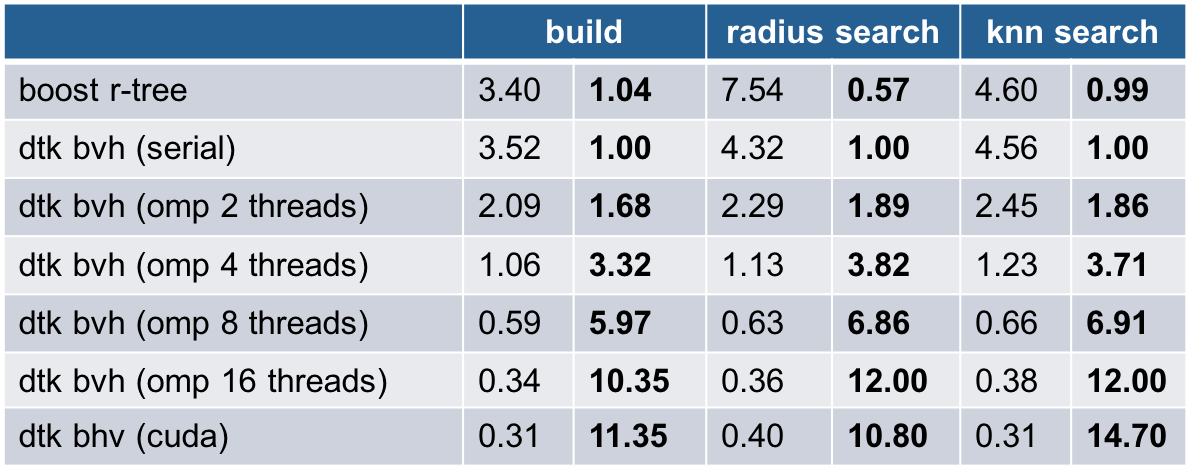
\includegraphics[width=3.0in]{projects/2.3.3-MathLibs/2.3.3.11-ALExa/dtk-gpu}
        \caption{\label{fig:dtk-gpu}DTK search performance relative to Boost with Intel Xeon E5-2698 and Nvidia P100. 10M points randomly distributed in a unit cube, 1M queries. The time is in seconds. Speedup in bold.}
\end{figure}

{\bf Tasmanian:} The infrastructure of Tasmanian has been upgraded to support
the broader ECP focus of the work.  GPU acceleration of sparse grid surrogates
has been implemented.  Tasmanian recently enabled the ExaStar project to
reduce the size of a large-memory table of neutrino opacities by 100X while
still preserving accuracy.

\begin{figure}[htb]
        \centering
        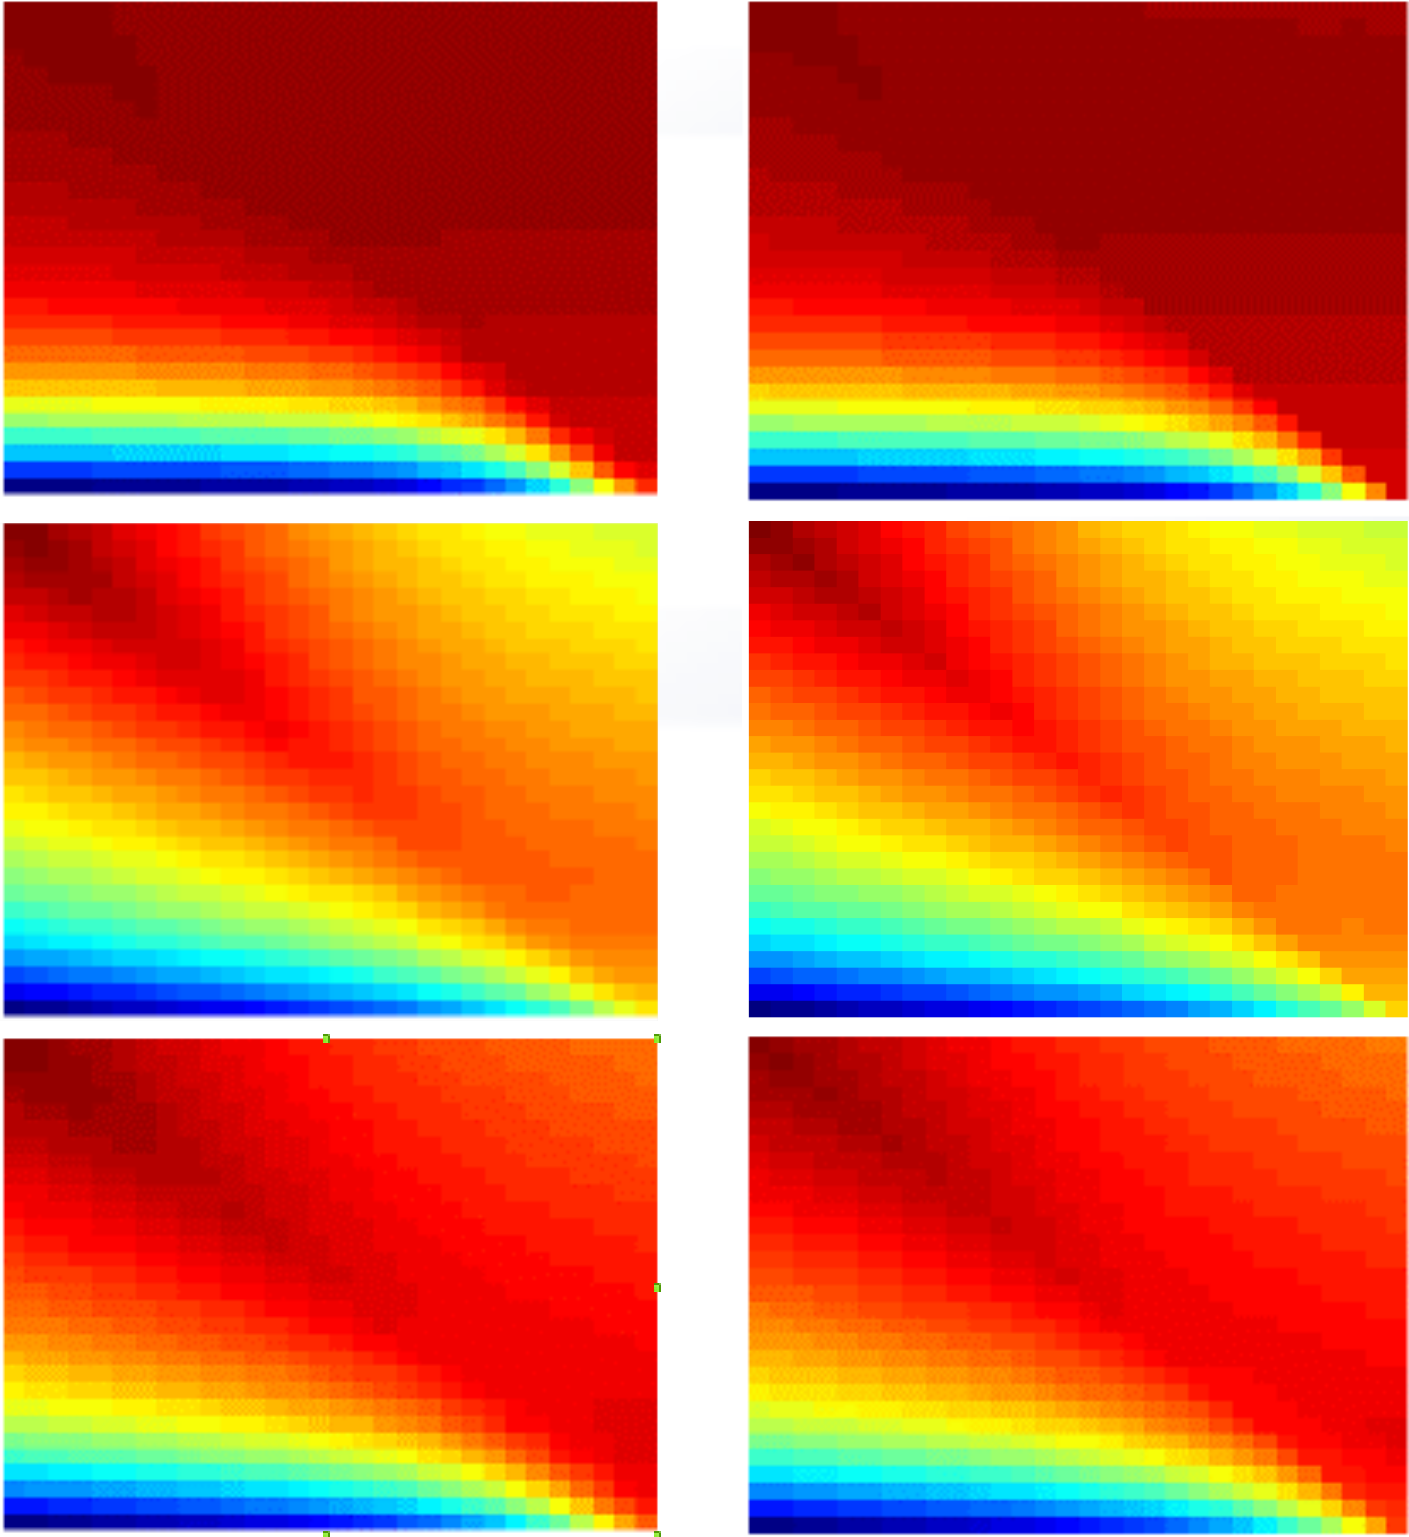
\includegraphics[width=1.5in]{projects/2.3.3-MathLibs/2.3.3.11-ALExa/tasmanian-gpu}
        \caption{\label{fig:tasmanian-gpu}Tasmanian approximation (right) of neutrino capacities (left).}
\end{figure}

%----------------------------------------

\paragraph{Next Steps}

\indent

{\bf DTK:} DTK search and communication capabilities will deployed in a new,
lightweight library, ArborX, to provide these ECP investments to a broader
user base.

{\bf Tasmanian:} Work will continue with the development of the asynchronous
construction methods that exploit the native sparse grids DAG hierarchy.

%----------------------------------------
